%!TEX root = *.tex
%%%%%%%%%%%%%%%%%%
% カウンタのリセット
\setcounter{figure}{0}
% 問題文
{%
\begin{wrapfigure}{r}{0.3\columnwidth}
  \vspace*{\baselineskip}
  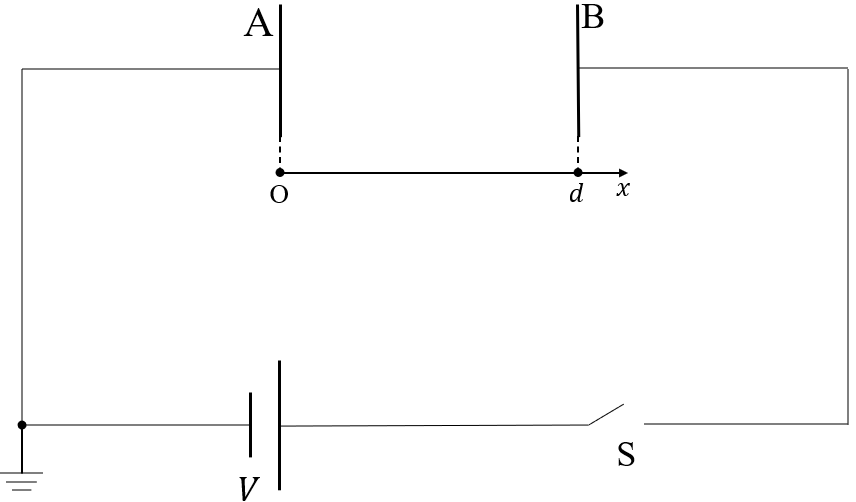
\includegraphics[width=0.3\columnwidth]{../graphs/jumon_108_1.png}
  \caption{}
\end{wrapfigure}
真空中で図1のように,2枚の薄い金属板A,Bを間隔\mbox{$d\unit{m}$}はなして配置した平行平板コンデンサーの両端に起電力\mbox{$V\unit{V}$}の電池とスイッチSがつないである.
$d$は金属板の大きさに対して十分に小さく,金属板の周辺部分の不均一さは無視できるとする.
金属板Aは接地してあり,その電位は$0\unit{V}$に保たれている.
図1のように金属板Aの位置を原点\O として金属板に垂直な方向に\x 軸をとる.
このコンデンサーの電気容量は$C\unit{F}$である.次の問いに答えよ.
\par}

スイッチSを閉じて十分に時間をおいた.

\begin{enumerate}[(1)]
  \setlength{\leftskip}{-1.5zw}
  \setlength{\itemindent}{1zw}\setlength{\labelsep}{0.5zw}
  \setlength{\labelwidth}{1zw}\setlength{\leftmargin}{1zw}
  \setlength{\itemsep}{0.5\baselineskip}
  \item このコンデンサーに蓄えられている静電エネルギーを答えよ.
  \item 金属板A,B間の座標\x における電位を図2に描け.
  \item 金属板A,B間の座標\x における電場の強さを図3に描け.
\end{enumerate}

\begin{figure}[H]
  \centering
  \begin{minipage}{0.4\columnwidth}
    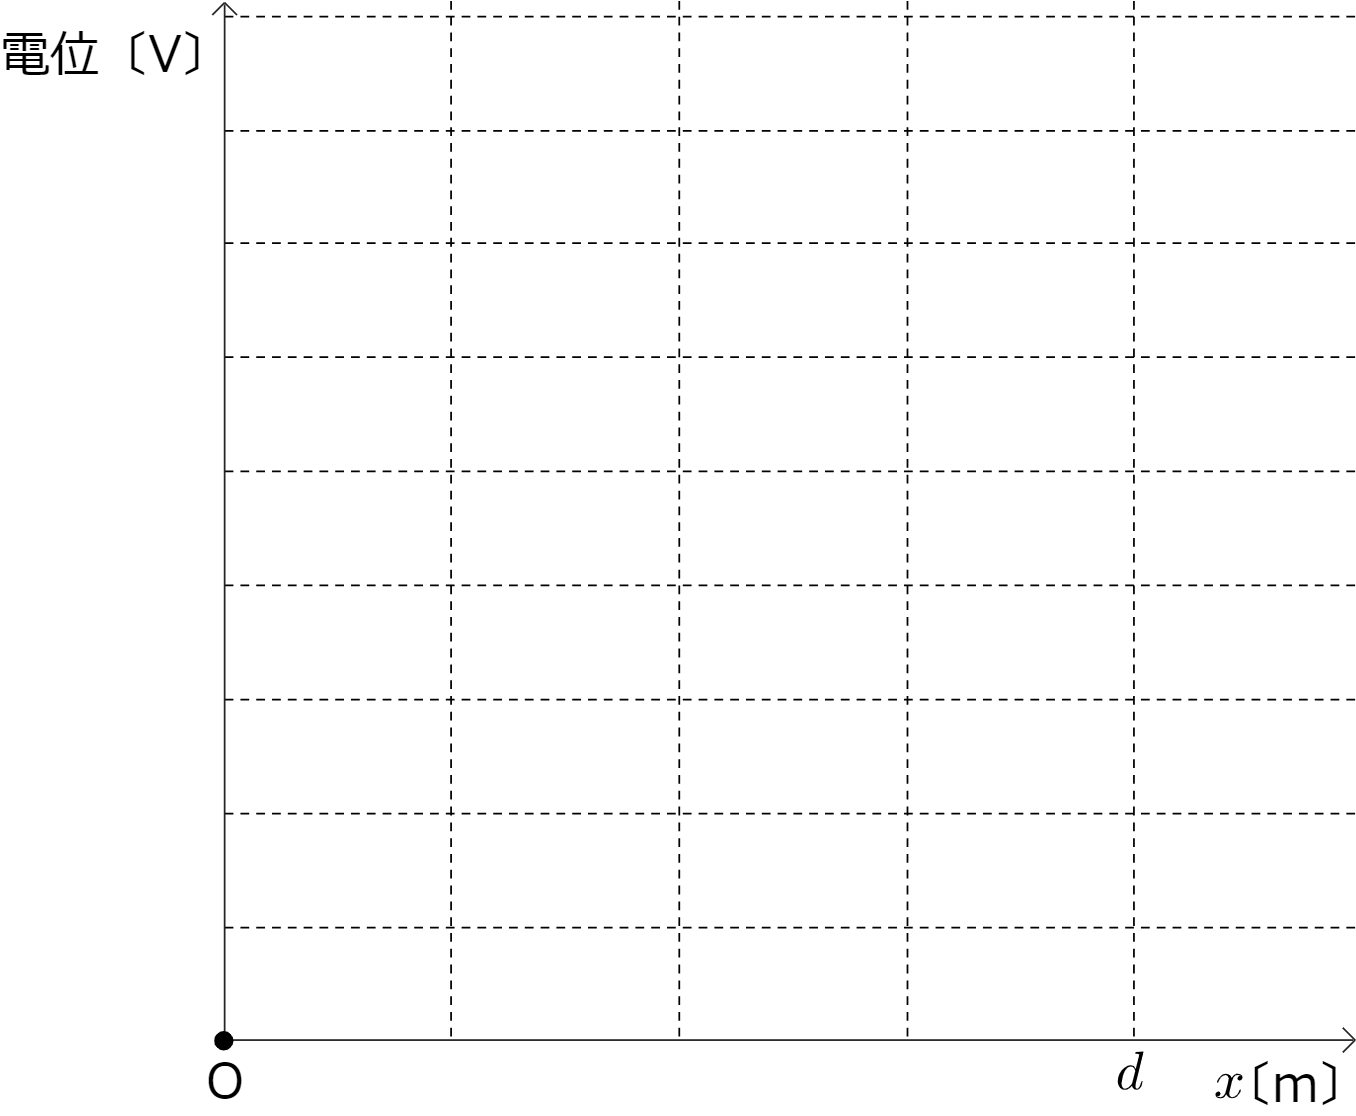
\includegraphics[width=\columnwidth]{../graphs/jumon_108_2.png}
    \caption{}
  \end{minipage}
  \begin{minipage}{0.4\columnwidth}
    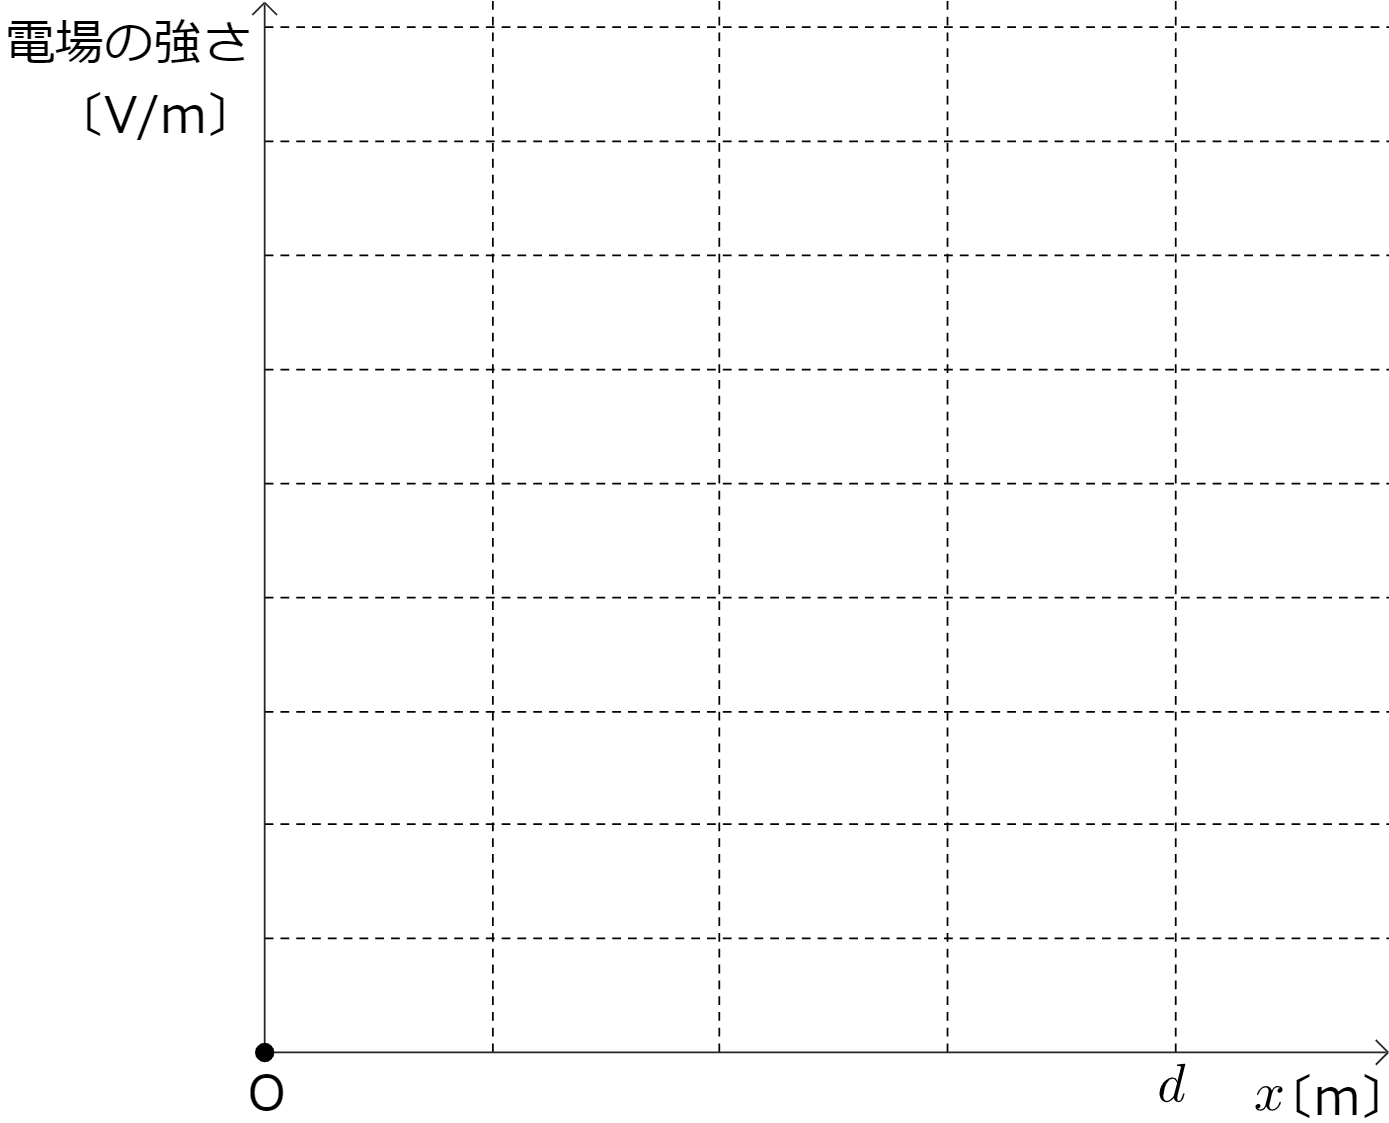
\includegraphics[width=\columnwidth]{../graphs/jumon_108_3.png}
    \caption{}
  \end{minipage}
\end{figure}

次にコンデンサーを完全に放電した.そして,スイッチSを開いた状態で図4のように金属板A,Bの間に厚さ$\dfrac{d}{2}\unit{m}$の金属板をA,Bそれぞれからの距離が等しくなるように挿入した.その後,スイッチSを閉じて十分に時間をおいた.
\begin{enumerate}[(1)]
  \setlength{\leftskip}{-1.5zw}
  \setlength{\itemindent}{1zw}\setlength{\labelsep}{0.5zw}
  \setlength{\labelwidth}{1zw}\setlength{\leftmargin}{1zw}
  \setlength{\itemsep}{0.5\baselineskip}
  \addtocounter{enumi}{3}
  \item このコンデンサーに蓄えられている電気量を答えよ.
  \item 金属板A,B間の座標\x における電位を図2に描き足せ.
  \item 金属板A,B間の座標\x における電場の強さを図3に描き足せ.
\end{enumerate}

\begin{figure}[H]
  \centering
  \begin{minipage}{0.3\columnwidth}
    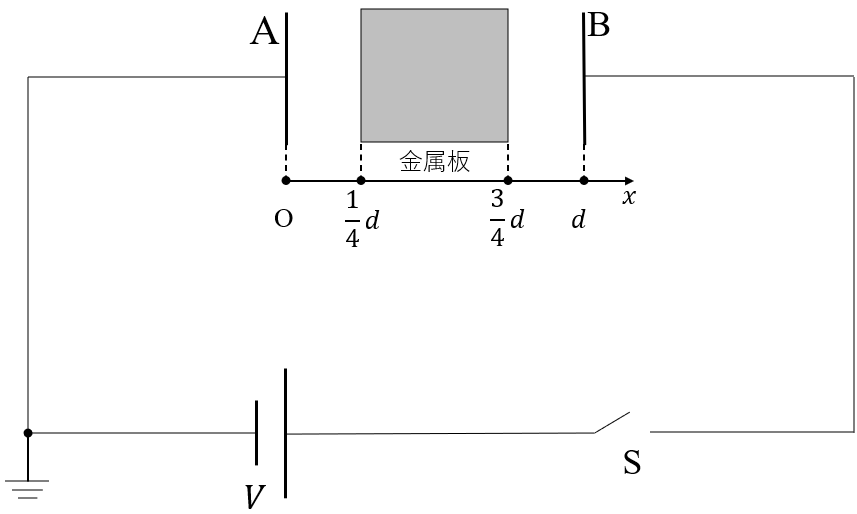
\includegraphics[width=\columnwidth]{../graphs/jumon_108_4.png}
    \caption{}
  \end{minipage}
  \begin{minipage}{0.3\columnwidth}
    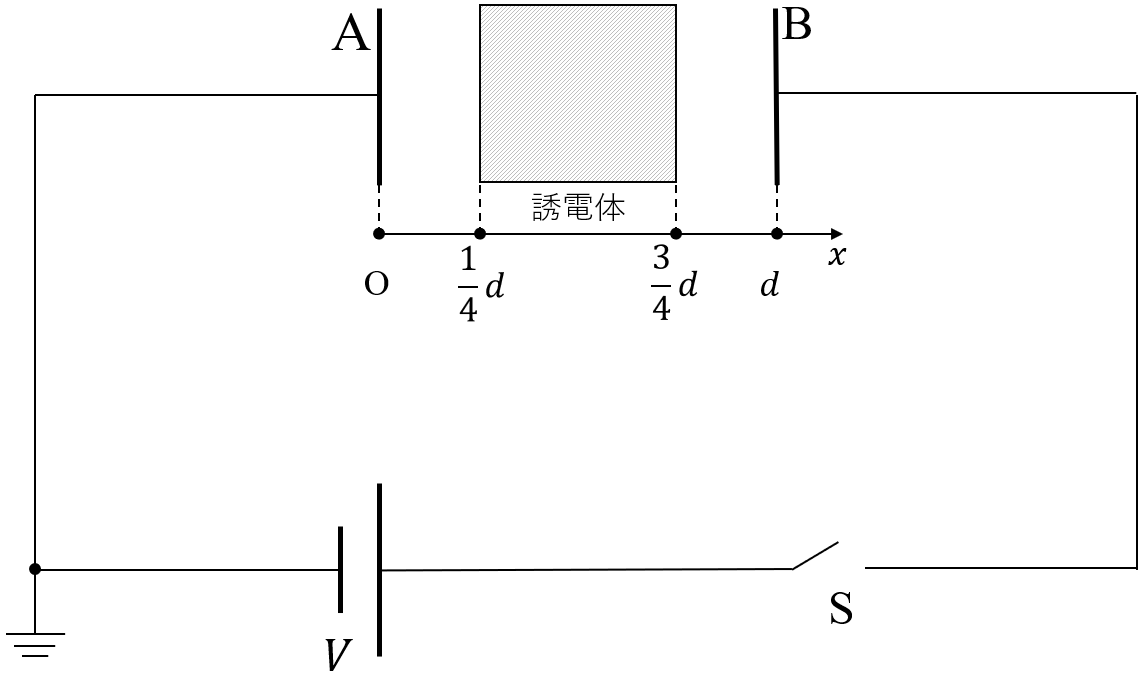
\includegraphics[width=\columnwidth]{../graphs/jumon_108_5.png}
    \caption{}
  \end{minipage}
  \begin{minipage}{0.3\columnwidth}
    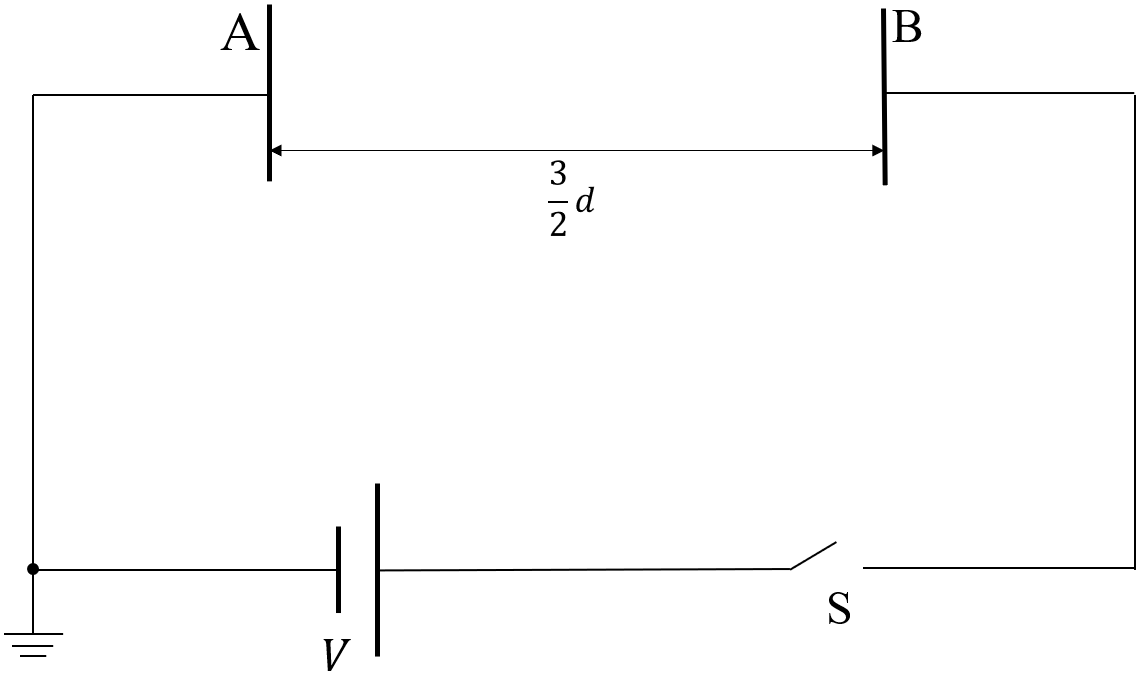
\includegraphics[width=\columnwidth]{../graphs/jumon_108_6.png}
    \caption{}
  \end{minipage}
\end{figure}

再びコンデンサーを完全に放電した.
そして,スイッチSを開いた状態で図5のように金属板A,Bの間に比誘電率が2で,
厚さが$\dfrac{d}{2}\unit{m}$の誘電体をA,Bそれぞれからの距離が等しくなるように挿入した.
その後,スイッチSを閉じて十分に時間をおいた.

\begin{enumerate}[(1)]
  \setlength{\leftskip}{-1.5zw}
  \setlength{\itemindent}{1zw}\setlength{\labelsep}{0.5zw}
  \setlength{\labelwidth}{1zw}\setlength{\leftmargin}{1zw}
  \setlength{\itemsep}{0.5\baselineskip}
  \addtocounter{enumi}{6}
  \item このコンデンサーに蓄えられている電気量を答えよ.
  \item 金属板A,B間の座標\x における電位を図2に描き足せ.
  \item 金属板A,B間の座標\x における電場の強さを図3に描き足せ.
\end{enumerate}

続いてスイッチSを開いた後に,金属板A,B間の距離を保ったまま誘電体を取り除いた.
\begin{enumerate}[(1)]
  \setlength{\leftskip}{-1.5zw}
  \setlength{\itemindent}{1zw}\setlength{\labelsep}{0.5zw}
  \setlength{\labelwidth}{1zw}\setlength{\leftmargin}{1zw}
  \setlength{\itemsep}{0.5\baselineskip}
  \addtocounter{enumi}{9}
  \item 誘電体を取り除くために要した仕事を答えよ.
\end{enumerate}

その後,図6のように金属板A,Bの間隔を$\dfrac{3}{2}d\unit{m}$に広げて十分に時間をおいた.
\begin{enumerate}[(1)]
  \setlength{\leftskip}{-1.5zw}
  \setlength{\itemindent}{1zw}\setlength{\labelsep}{0.5zw}
  \setlength{\labelwidth}{1zw}\setlength{\leftmargin}{1zw}
  \setlength{\itemsep}{0.5\baselineskip}
  \addtocounter{enumi}{10}
  \item このときの金属板A,B間の電位差を答えよ.
\end{enumerate}

% メモ
\begin{comment}

\end{comment}


%%%%%%%%%%%%%%%%%%
